\documentclass[10pt]{article}
\usepackage[a4paper,margin=1.7cm,top=1.5cm,bottom=1.6cm]{geometry}
\usepackage[T1]{fontenc}
\usepackage{lmodern,microtype,graphicx,booktabs,array,xcolor,amsmath}
\usepackage[font=small,labelfont=bf,skip=3pt]{caption}
\usepackage[colorlinks=true,linkcolor=black,citecolor=black,urlcolor={rgb:blue,3;black,2}]{hyperref}
\setlength{\parskip}{2pt}\setlength{\parindent}{0pt}
\renewcommand{\arraystretch}{1.08}
\newcommand{\sect}[1]{\par\vspace{5pt}{\large\bfseries #1}\par\nobreak\vspace{1pt}\nobreak}
\newcommand{\ci}[2]{\,{\footnotesize[#1,\,#2]}}

\begin{document}
{\LARGE\bfseries Rescue Router: few-shot flood mapping and rescue routing with Chameleon}\par\vspace{2pt}
{\large Marlen Melis \quad 20260876 \quad KAIST AIC200 mini-project \quad \textbf{Track A + Track B}}\par
\vspace{3pt}
\textbf{Summary.} We adapt Chameleon to map flooded roads and buildings in drone photos from \textbf{50 labelled photos}
(Track A) and build a rescue router, a web viewer and a Gradio app on its predicted maps (Track B). On the full
448-photo FloodNet test set the model reaches \textbf{mIoU .472}\ci{.437}{.506} (5 classes, 95\,\% bootstrap CI); the
router finds the houses that are cut off by road with \textbf{F1 .759}\ci{.638}{.856}. A fully supervised PSPNet trained on
1,445 labels reaches .848 on the same classes, so this is a fast first map, not a replacement for full labelling.

\sect{1\quad Problem and motivation}
On 8 Aug 2022 Seoul recorded 141.5\,mm of rain in one hour, the most since records began in 1907, and streets in
Gangnam turned into rivers~\cite{seoul}. On 15 Jul 2023 an embankment failure flooded the Gungpyeong 2 underpass in
Osong within minutes: 17 vehicles were trapped and 14 people died~\cite{osong}. In the first hours of such an event,
rescue coordinators need one answer per street and per house: \emph{can a truck get there, does it need a boat, or
is it cut off?} Drones deliver photos within the hour, but turning photos into a map takes people: pixel labels for
the two public post-hurricane datasets took about \textbf{one hour per photo}~\cite{floodnet,rescuenet}, and a
supervised segmentation model needs the 1,445 labelled photos of FloodNet's training split. Our question: how good is a
map adapted from a few labelled photos of the \emph{new} disaster (50 photos $\approx$ 50 labeller-hours, 3.5\,\% of
FloodNet's training labels), and is it good enough to route rescue teams, if the system says how much to trust it?

\sect{2\quad Formulation as structured prediction}
\begin{minipage}[t]{0.52\textwidth}\vspace{0pt}
Each 768$\times$576 photo gets a \textbf{dense label with $C=5$ channels} (right). The label is a one-hot
$Y\in\{0,1\}^{5\times H\times W}$; pixels of every other class (tree, grass, vehicle, pool, background) are 0 in all five
channels and are decoded as \emph{other}; the mask $M$ is 1 except on unlabelled pixels. Chameleon predicts one sigmoid
map per channel (binary cross-entropy). A pixel takes the channel with the largest $p_c/\tau_c$ among those with
$p_c\ge\tau_c$, else \emph{other}; $\tau_c=0.5$, or per-channel values tuned on 30 validation photos.
\end{minipage}\hfill
\begin{minipage}[t]{0.45\textwidth}\vspace{0pt}\small
\begin{tabular}{@{}cll@{}}\toprule
ch & FloodNet / RescueNet class & role in routing\\\midrule
0 & road clear & truck\\
1 & road flooded / road blocked & boat, no truck\\
2 & building flooded / intact & target, obstacle\\
3 & building dry / damaged & target, obstacle\\
4 & water & boat\\\bottomrule
\end{tabular}
\end{minipage}
\vspace{2pt}

The channels are chosen for the consumer, a \textbf{router} (Track B). Its input is the cell grid of the decoded map
(4$\times$4-pixel cells) plus the water probability $p_\text{wet}=p_1+p_4$; its output is a status per house
(\textsc{truck}, \textsc{boat}, \textsc{foot}, \textsc{isolated}) and a route (\S4). Inference tiles the photo with
384-px tiles at stride 192 (6 tiles) and blends them with Gaussian weights. \textbf{Rejected alternatives:} all 10
FloodNet classes (spends 50 shots on trees and grass the router does not need); a single ``passable'' channel (no
targets, no boat leg); regressing a cost map (no labels exist); trees as obstacles (canopy hides real roads from
above); pools as water (pools are not routes).

\sect{3\quad Data and resources}
\textbf{FloodNet}~\cite{floodnet} (Hurricane Harvey, Texas 2017; 2,343 drone photos, 4000$\times$3000, split
1,445\,/\,450\,/\,448; CDLA-Permissive-1.0, \url{https://github.com/BinaLab/FloodNet-Supervised_v1.0}).
\textbf{RescueNet}~\cite{rescuenet} (Hurricane Michael, Florida 2018; 4,494 photos; CC0 on figshare,
\href{https://doi.org/10.6084/m9.figshare.c.6647354}{doi:10.6084/m9.figshare.c.6647354}; road blocked = blocked by water,
sand or debris; building intact = no or minor damage). \textbf{We labelled nothing ourselves}: all labels are the
datasets'. Photos were area-downsampled to 768$\times$576 (labels nearest-neighbour; 57 FloodNet photos needed their
EXIF 180$^\circ$ rotation applied). Splits were fixed before choosing supports and are checked by SHA-256 in the
notebook: \textbf{supports} = 50 FloodNet training photos, chosen stratified so the rare flooded classes appear, and
nested (the $k$-shot set is the first $k$); RescueNet supports come from its validation split. \textbf{val30} (30 val
photos) selects checkpoints, decodes and router gates. \textbf{eval100} (100 test photos, half with flooding) gives the
learning curve; the \textbf{full test} (448) gives the headline. We checked for test photos that show the same ground
as a support photo (ORB + RANSAC): 14 of 448 do; removing them changes mIoU by $\le$.004.

\textbf{Pretrained weights.} (1) The \textbf{Chameleon} meta-trained generalist checkpoint~\cite{chameleon} distributed
by the course (\url{https://github.com/GitGyun/AIC200-Project-StructuredPrediction}, shared Drive folder; model code
\url{https://github.com/GitGyun/chameleon}). It contains (2) its BEiT-v2-Large image encoder~\cite{beitv2} and (3) its
ViT-L label encoder and DPT-style decoder as released by the Chameleon authors. No other pretrained model is used.
\textbf{Compute:} all GPU work ran on 16-GB NVIDIA T4s on Kaggle, about 17 GPU-hours in total.

\sect{4\quad Method and experimental setup}
\begin{minipage}[t]{0.50\textwidth}\vspace{0pt}
\textbf{Fine-tuning} (the same recipe for every run, sized so a 50-shot run fits a T4; right). Only the parameters the
starter fine-tunes are trained (biases, the matching temperature, a LayerNorm), so a checkpoint is $\approx$5\,MB.
Validation on val30 every 250 steps (every 500 on saved snapshots at 50 shots, where inference does not fit next to the
training state); the best step is kept. Runs: FloodNet 1, 5, 10, 20, 50 shots and RescueNet 20, 50 (seed 0).
\textbf{Inference:} fp16, 6 tiles, 17\,s per photo at 50 shots (12\,GB). \textbf{Decode tuning} on val30:
coordinate ascent on per-channel $\tau$ with drivable-road precision not allowed to drop (a false ``clear'' sends a
truck into water), then optional building-level rules (one flooded/dry label per building).
\end{minipage}\hfill
\begin{minipage}[t]{0.47\textwidth}\vspace{0pt}\small\setlength{\tabcolsep}{4pt}
\begin{tabular}{@{}ll@{}}\toprule
input & 384\,px crops (side 320--480\,px)\\
augment & flips, rot90, bright./contrast 0.2\\
support (inference) & best 384\,px window\\
batch; optimiser & 2; Adam, lr $10^{-3}$ cosine, no decay\\
steps & 1,000 ($\le$10 shots), 2,000 (20, 50)\\
precision & fp16 + scaler, grad.\ ckpt.\\
speed (T4) & 3.6--4.1\,s/step, 10--13.5\,GB\\\bottomrule
\end{tabular}
\end{minipage}
\vspace{3pt}

\textbf{Router} (Dijkstra over (cell, mode) states; modes go truck $\rightarrow$ boat $\rightarrow$ on foot, never back into
a vehicle). A truck drives on clear road at cost 1 per cell, plus $5\,p_\text{wet}$ (risk-aware), or on dry land at
4$\times$; on a \emph{predicted} map only where $p_\text{wet}<g$ (\textbf{off-road gate}, $g=0.3$ FloodNet, 0.2
RescueNet, each tuned on val30). A boat needs water or flooded road (3$\times$, launch +40); the last stretch can be
walked (8$\times$, +10 to get out). Vehicles have a width (truck 2.5\,m, boat 1.6\,m; ground scale from the cars in the
photo), parked cars do not block a road, boats pass under tree canopy, and nothing squeezes diagonally between two
obstacles. The \textbf{labelled map} is the same router on the human labels: the datasets label pixels, not
reachability, so this is our reference, not ground truth. We score the houses \textbf{cut off by road} (status $\ne$
\textsc{truck}) on the predicted map against the labelled map (P, R, F1). \textbf{Confidence tiers:} each prediction is
routed again with a cautious gate (0.1 FloodNet, 0.15 RescueNet, chosen on val30 as the largest gate whose
truck-reachable houses are $\ge$99\,\% correct); a house a truck still reaches is \emph{confident}, else
\emph{check first}. The \textbf{system}: a web viewer (Leaflet; the router ported to JavaScript and bit-exact with
Python on all 200 scenes) and a Gradio app that runs the model live on an uploaded photo.

\sect{5\quad Results and analysis}
\begin{minipage}[t]{0.40\textwidth}\vspace{0pt}
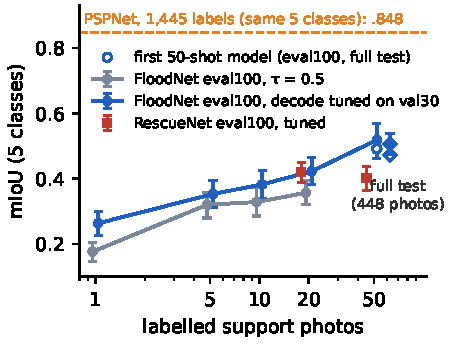
\includegraphics[width=\linewidth]{figs/curve.pdf}
\captionof{figure}{Learning curve (eval100, 95\,\% CIs over photos); diamonds: full test.}\label{fig:curve}
\end{minipage}\hfill
\begin{minipage}[t]{0.57\textwidth}\vspace{0pt}\small\setlength{\tabcolsep}{3.5pt}
\begin{tabular}{@{}lcccccc@{}}\toprule
IoU (full test) & labels & r.\,clear & r.\,flood & b.\,flood & b.\,dry & water\\\midrule
ours, $\tau$ 0.5 & 50 & .501 & .293 & .558 & .298 & .450\\
ours, tuned & 50 & .544 & .291 & .577 & .500 & .448\\
ENet~\cite{floodnet} & 1,445 & .484 & .125 & .069 & .474 & .490\\
DeepLabV3+~\cite{floodnet} & 1,445 & .702 & .520 & .327 & .728 & .752\\
PSPNet~\cite{floodnet} & 1,445 & .912 & .822 & .689 & .898 & .920\\\bottomrule
\end{tabular}
\captionof{table}{Per class, full 448-photo test. Baselines: FloodNet paper (10 classes, 713$\times$713); our 5-channel
decode avoids tree/grass confusions, which may favour us slightly.}\label{tab:base}
\end{minipage}
\vspace{3pt}

\textbf{Segmentation (Track A).} The curve rises from .26 (1 photo) to .49 (50 photos) on eval100 with the tuned decode
(Fig.~\ref{fig:curve}); paired bootstrap differences show real gains from 1$\rightarrow$5 (+.14\ci{+.10}{+.18}) and
20$\rightarrow$50 (+.10\ci{+.06}{+.14}, $\tau$ 0.5), but 5$\rightarrow$10 is indistinguishable from zero
(+.01\ci{$-$.03}{+.05}). On the full test the 50-shot model reaches \textbf{.420}\ci{.386}{.455} at $\tau$ 0.5 and
\textbf{.472}\ci{.437}{.506} tuned (Table~\ref{tab:base}): above ENet on 4 of 5 classes and above DeepLabV3+ on flooded
buildings, far below PSPNet; \textbf{flooded roads are the gap} (.29 vs .82). The model never learned a flooded/dry
signal for buildings (per-building AUC $\approx$0.5); a rule tuned on val30 (``flooded if water lies within
$\sim$10\,m'') fixes dry buildings at 5--20 shots. \textbf{Cross-disaster:} the FloodNet model applied to RescueNet
with zero RescueNet labels reaches about half of what 20 RescueNet labels give (mean road/building/water IoU .32 vs .63):
a new disaster needs its own few labels. RescueNet 20-shot: .421 (eval100, tuned); 50 shots did not help (.402).
\textbf{Failure analysis} (16 worst eval100 photos, tagged by eye): the dangerous error is \textbf{shallow or muddy water
decoded as dry land}; 92\,\% of the labelled-water cells on predicted truck routes had been crossed as dry off-road land
(median $p_\text{wet}$ .21), which is why the off-road gate exists. Most other errors are benign for routing
(water vs flooded road, both boat cells) or are label ambiguities (bridges labelled ``flooded road'').

\textbf{Routing (Track B).} Houses cut off by road, prediction vs labelled map: FloodNet full test (1,232 houses)
P .847, R .687, \textbf{F1 .759}\ci{.638}{.856}; eval100 \textbf{.835}\ci{.752}{.899}; RescueNet 20-shot eval100
\textbf{.818}\ci{.524}{.966} (only 25 cut-off houses). The off-road gate lifts val30 F1 from .556 to .980 and eval100
from .737 to .835; vehicle widths add .802$\rightarrow$.835 (FloodNet eval100). Statuses do not depend on the cost
values at all (14 cost changes, 0 status changes), and F1 stays within .78--.86 when the gate, cell size, goal ring or
vehicle widths change. \textbf{Confidence tiers:} of 490 houses the prediction calls truck-reachable on FloodNet eval100,
the 301 \emph{confident} ones are \textbf{98.7\,\%} truly truck-reachable, the 189 \emph{check first} only 74\,\%; in the
honest-failure scene 7241 all 6 wrongly truck-reachable houses are \emph{check first}. Buildings found on the predicted
map match labelled buildings with F1 .85 (RescueNet .63). Test-time flips (4 views) were tried and \textbf{not adopted}:
with their own val30-tuned decode the full test fell to .455.

\textbf{System.} Fig.~\ref{fig:routes} shows the router on a predicted and a labelled map. The notebook runs end to end
on a fresh T4 in 26 minutes and \textbf{recomputes the 50- and 20-shot models live: identical to the stored predictions}
(maximum difference 0), then routes an uploaded photo through the app in 16\,s. The viewer shows all 200 eval100 photos,
animated routes, minutes and metres, and the water probability behind each ``check first''.

\begin{figure}[h]\centering
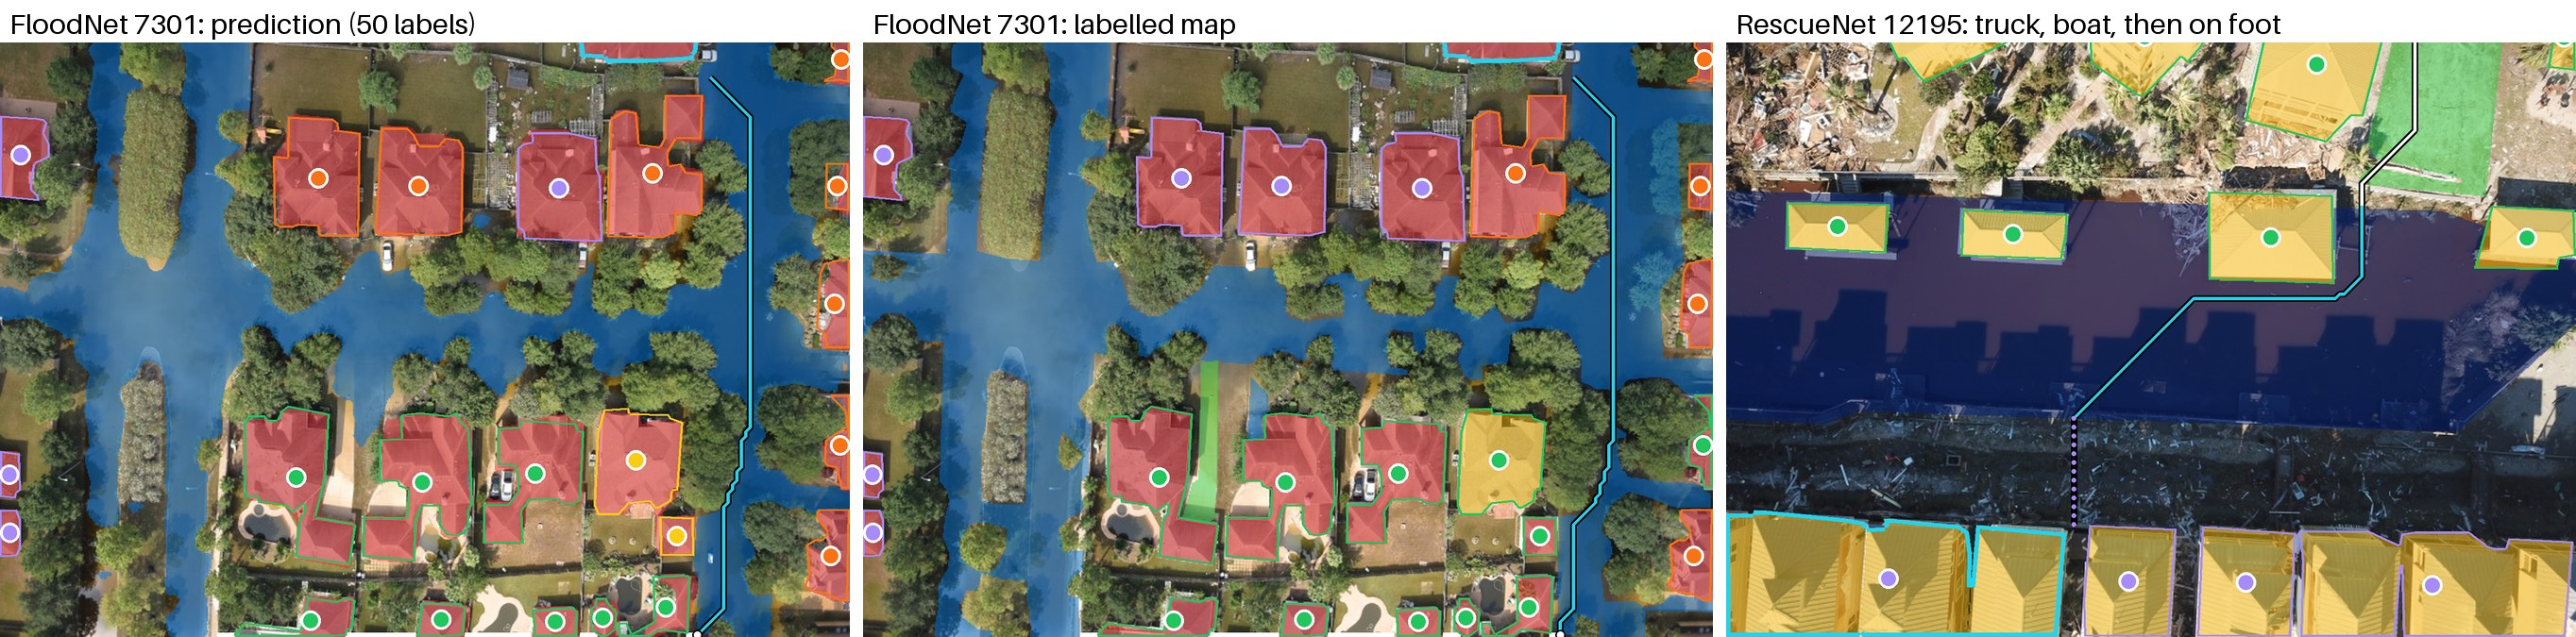
\includegraphics[width=\linewidth]{figs/routes.jpg}
\caption{Badges: house status (green truck, orange boat, violet on foot, yellow \emph{check first}); route: white truck,
cyan boat, violet dots on foot. Left/middle: the same flooded street, prediction vs labelled map; the selected house
needs a boat on both. Right: RescueNet canal row, truck $\rightarrow$ boat across the canal $\rightarrow$ on foot.}\label{fig:routes}
\end{figure}\vspace{-6pt}

\textbf{Limitations.} US hurricane suburbs are not Korean urban floods (dense blocks, underpasses invisible from above);
single nadir frames without georeferencing or mosaics; the labelled map encodes our router's assumptions, not
field-checked access; one seed per point; val30 is reused for checkpoints, decodes and gates (eval100 and the full test
were not used for any choice); minutes and metres are rough estimates.

\renewcommand{\refname}{\large References}
\begingroup\small
\begin{thebibliography}{9}\setlength{\itemsep}{0pt}
\bibitem{chameleon} D.~Kim, S.~Cho, S.~Kim, C.~Luo, S.~Hong. \emph{Chameleon: A Data-Efficient Generalist for Dense Visual Prediction in the Wild}. ECCV 2024. arXiv:2404.18459; \url{https://github.com/GitGyun/chameleon}.
\bibitem{floodnet} M.~Rahnemoonfar, T.~Chowdhury, A.~Sarkar et al. \emph{FloodNet: A High Resolution Aerial Imagery Dataset for Post Flood Scene Understanding}. IEEE Access 9, 2021. arXiv:2012.02951.
\bibitem{rescuenet} M.~Rahnemoonfar, T.~Chowdhury, R.~Murphy. \emph{RescueNet: A High Resolution UAV Semantic Segmentation Dataset for Natural Disaster Damage Assessment}. Scientific Data 10, 2023. doi:10.1038/s41597-023-02799-4.
\bibitem{beitv2} Z.~Peng, L.~Dong, H.~Bao et al. \emph{BEiT v2: Masked Image Modeling with Vector-Quantized Visual Tokenizers}. arXiv:2208.06366, 2022.
\bibitem{seoul} NPR, \emph{Historic rainfall turns Seoul's roads into rivers and leaves 8 dead}, 9 Aug 2022. \url{https://www.npr.org/2022/08/09/1116455746/historic-rainfall-turns-seouls-roads-into-rivers-and-leaves-8-dead}.
\bibitem{osong} The Korea Times, \emph{50 dead or missing in downpours after 5 more bodies recovered from underground road}, 18 Jul 2023. \url{https://www.koreatimes.co.kr/www/nation/2023/07/281_355125.html}.
\end{thebibliography}
\par Code, data bundle and every reported number: the notebook \texttt{20260876\_MarlenMelis\_code.ipynb} and \texttt{src/rebuild\_all.py}.
\endgroup
\end{document}
